\documentclass[../TFG_Report.tex]{subfiles}
 
\begin{document}
	
	In this section, the design approach that will be followed is discussed and justified. 

\subsection{General architecture}

The general architecture of the wind turbine will be based on the tendencies seen in the state of the market. \\

\begin{enumerate}


\item \textbf{Horizontal axis, upwind wind turbine:} The horizontal axis option is selected because it is the most used and studied. Although the vertical axis is growing in importance, the classic concept will be chosen. The rotor position will also follow the usual convention: an upwind wind turbine will be selected. A downwind concept would simplify the yaw stabilization system, but it could also lead to big fatigue loads and dangerous aeroelastic coupling. As the loads analysis that will be performed does not involve a detailed aerolastic temporal analysis, it is desirable to avoid this possible problems since the beginning. \\

\item  \textbf{Three blades:} In the figure \ref{fig:cpnumberblades} the influence of the number of blades on the optimal tip speed ratio and maximum power coefficient has been shown. Following the same reasoning that was discussed there, it is desirable to increase the power coefficient by selecting a higher number of blades, but the cost in material and forces of this option are the main drawback. In a small wind turbine, the effect of the tip speed ratio should be taken into account. Because of the small radius, if a high tip speed ratio is desired, the angular velocity of the blades should be very high. Thus, the corresponding centrifugal forces will increase as well. An approximated magnitude of this effect is represented in the following figure:

\begin{figure}[h!]
	\centering
	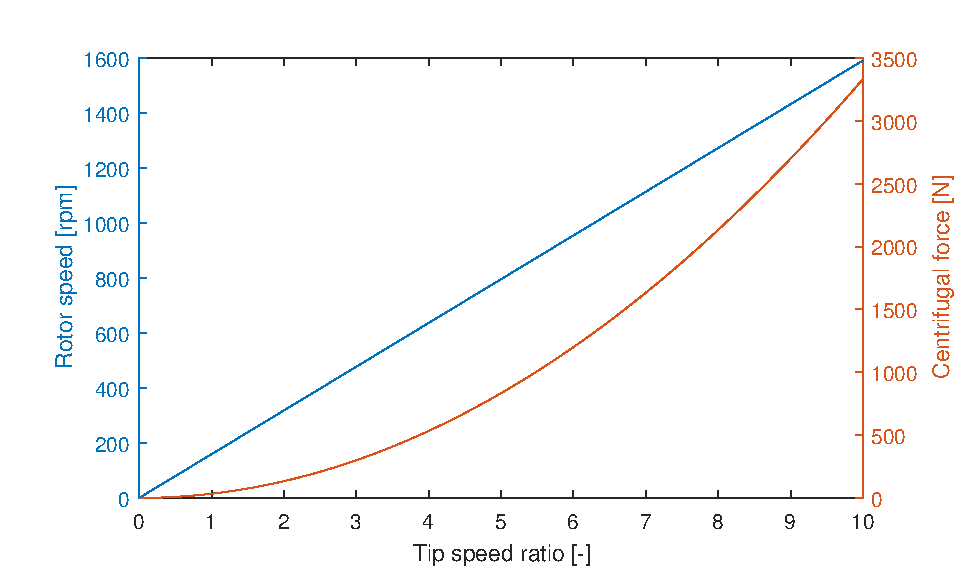
\includegraphics[width=0.8\linewidth]{Images/Lambda_influence_axial_force}
	\caption[Influence of the tip speed ratio on the centrifugal force]{Influence of the tip speed ratio on the centrifugal force. \\
		Values estimated at 10 m/s for a wind turbine of 1.2 m diameter.}
	\label{fig:lambdainfluenceaxialforce}  
\end{figure}
\FloatBarrier

%%FER LA GRÀFICA ANTERIOR AMB EL DIÀMETRE DEFINITIU????

This illustrates the importance of being able to operate at the lower tip speed ratio possible. This is why three blades are preferable rather than two, specially in this case. When it comes to change from three to four blades, the decision is not that clear. The increase in power coefficient and the decrease in rotor speed are lower, and the rotor instability might be a source of problems. The hub design is also compromised (more blades to join, more space needed), and the blade cost is increased again. Thus, this option is discarded and three blades will be the final choice, following the trend of the market. \\

\item \textbf{1.0 m rotor diameter:} The rotor diameter selection is constrained by the possibilities of the 3D printer that will be used. The printer characteristics will be exposed more deeply in the section \ref{Section_printer_character}. The biggest restriction that it imposes is the available printing space: 220x220x250 mm, which means that the blades will have to be built out of more than one piece. It can be anticipated that the join between the different parts will be an added difficulty to the design, so it may be helpful to reduce the amount of parts. A blade made of two pieces is selected. This option will keep the material cost as low as possible but will still involve the challenge of joining two different parts, and the study and methodology used could be extrapolated to even more parts. \\

For the first design, it will be assumed that each piece will be 25 cm long, so the blade radius will be 50 cm. However, this assumption neglects the presence of the hub, which would "add" diameter, and also ignores any radial extra space used for the joint, what would "subtract" diameter. \\

\item \textbf{Entirely passive control system: } Large commercial wind turbines count with torque and pitch control systems, which allows them to reduce loads, have a big range of operation capabilities and ultimately increase the power production. On the other hand, small wind turbines seldom have a pitch controller, and the torque controller is not a clearly dominant option. For this project, none of them will be developed. \\

Although a torque controller would simplify the aerodynamic design (as the rotor speed could be practically selected for each wind speed), there are two major drawbacks. First, the hardware would increase in cost (a different generator plus the variable speed drive) and the software would increase in complexity. Second, it is desirable to come up with a design that can be easily reproduced for anyone with access to a 3D printer. If a control system is included, with both the hardware and software it involves, it will be likely more difficult to replicate. \\


\item \textbf{Over-speed control by furling: } This characteristic is highly related to the preceding one. An over-speed control is needed even though there is not any controller for the normal operation. This will allow the turbine to operate safely under extreme wind conditions, which will increase its life span and simplify the structural requirements. There are two main options for a passive over-speed control: \\

The first option is a furling mechanism, which turns the rotor away from the incoming wind flow. The rotor can be either rotated around the tower axis or around the axis perpendicular to the tower and contained in the rotor plane. This rotation is achieved through the higher thrust obtained at higher wind speeds, and the system should be designed in a way that this higher force creates a moment around the above-mentioned axis. The furling mechanism should be dimensioned so that the deviation occurs at the desired wind speed. \\

%%THIS WILL BE DESCRIBED MORE DEEPLY IN... CITAR EL CAPITOL ON ES DIMENSIONA EL FURLING

The second option is a passive stall mechanism, which simply uses the reduction in lift coefficient and the increase in drag coefficient in the post-stall region to create a ceiling in the power level as the wind speed increases. \\

The passive stall mechanism is a simpler option. However, it imposes big restrictions in the blade geometry, and it creates big uncertainties in the aerodynamic post-stall behavior. Most importantly, it is a requirement for applying this option that the angle of attack increases with the wind speed. In the section \ref{sec:design_challenge} it can be seen that this is not meet. Due to all these disadvantages, a furling mechanism is selected. \\


\item \textbf{Direct drive:} In the state of the market it has been seen that the tendency of the market is to avoid the use of gearbox, which adds weight, mechanical complication and decreases the efficiency. This preference will also be followed for this project. \\

\item \textbf{Permanent magnet generator: } Again, the market standard will be followed to select the generator type. %%MUST BE COMPLETED
	 
\end{enumerate}


%%  número de pales, diámetre rotor?


\subsection{Design procedure}

In a wind turbine almost everything is coupled. Therefore, is difficult to separate and design each part separately. To obtain a complete design that takes into account all the different parts, a iterative process should be made. The following figure shows the procedure that will be followed, as well as the different parts where the design can be divided into.  \\









	
	
\end{document}